\documentclass[a4paper]{article}

\usepackage[english]{babel}
\usepackage[utf8]{inputenc}
\usepackage[titletoc, toc]{appendix}
\usepackage{amsmath}
\usepackage{amsfonts}
\usepackage{graphicx}
\usepackage{mdframed}
\usepackage{cancel}
\usepackage{caption}
\usepackage{lipsum}
\usepackage{listings}
\usepackage{float}
\usepackage[colorinlistoftodos]{todonotes}

\title{Uncertainty Quantification (ACM41000) \\ Mini Project 2}

\author{Ian Towey \\ \\ 04128591}

\date{\today}

\lstdefinestyle{custom_py_style}{
  belowcaptionskip=1\baselineskip,
  breaklines=true,
  frame=L,
  xleftmargin=\parindent,
  language=Python,
  showstringspaces=false,
  basicstyle=\footnotesize\ttfamily,
  keywordstyle=\bfseries\color{green!40!black},
  commentstyle=\itshape\color{purple!40!black},
  identifierstyle=\color{blue},
  stringstyle=\color{orange}
}



% Number the subsubsections and include them in the TOC
\setcounter{secnumdepth}{3}
\setcounter{tocdepth}{3}
% \setcounter{section}{-1}

% Partial derivative
\newcommand*{\pd}[3][]{\ensuremath{\frac{\partial^{#1} #2}{\partial #3}}}

\newenvironment{aside}
  {\begin{mdframed}[style=0,%
      leftline=false,rightline=false,leftmargin=2em,rightmargin=2em,%
          innerleftmargin=0pt,innerrightmargin=0pt,linewidth=0.5pt,%
      skipabove=7pt,skipbelow=7pt]\footnotesize}
  {\end{mdframed}}

\begin{document}

  \maketitle

  \begin{abstract}
    Analytic and numerical analysis of the heat / diffusion equation.
  \end{abstract}

\tableofcontents
\newpage

\section{Introduction}
\label{sec:introduction}	

\section{Mixed Inhomogenous Boundary Conditions}
Breaking up the equation into two parts

\begin{equation}
u(x,t) = u_{hom}(x,t) + u_{PI}(x,t) 
\end{equation}
\subsection{$u_{hom}(x,t)$ solution with mixed homogenous boundary conditions}

\begin{equation}
\pd{u}{t}=D\pd[2]{u}{x^2} \hspace{15mm} x \in (0, L)
\end{equation}
Initial Conditions 
\begin{equation}
u(x,t = 0) = f(x) 
\end{equation}
Mixed homogenous boundary conditions
\begin{equation}
u(x = 0, t > 0) = u_{x}(x = L, t > 0) = 0
\end{equation}
Using the separation of variables method $u(x, t) = X(x)T(t)$
\begin{align*}
\pd{X(x)T(t)}{t} &= D\pd[2]{X(x)T(t)}{x^2} \\
\vspace{15mm}
\frac{1}{T(t)}\pd{T(t)}{t} &= D\frac{1}{X(x)}\pd[2]{X(x)}{x^2}
\end{align*}
LHS is a function of $T(t)$ only and the RHS is a function of $X(x)$ only. This means LHS = RHS = Constants 
\begin{align*}
\frac{1}{T(t)}\pd{T(t)}{t} = D\frac{1}{X(x)}\pd[2]{X(x)}{x^2} = -\lambda D 
\end{align*}
This produces the two following equations which can solved separately and recombined for the final solution
\begin{align}
\frac{1}{T(t)}\pd{T(t)}{t} &= -\lambda D \\
D \frac{1}{X(x)}\pd[2]{X(x)}{x^2} &= -\lambda D 
\end{align}

\subsubsection{Solve for $X(x)$}
Rearranging equation 6
\begin{align*}
\bcancel{D} \pd[2]{X(x)}{x^2} + \lambda X(x) \bcancel{D} = 0
\end{align*}
This is a second order linear homogenous ODE with constant coefficients. 
This can be seen as the solution of a quadratic of the form 
\begin{equation*}
 \Psi^{2} + \lambda \Psi = 0
\end{equation*}
Solutions to this quadratic are
\begin{align*}
 \Psi &= 0 \\
 \Psi &= \lambda
\end{align*}
Ignoring the $\Psi = 0$ solution and focusing on the $\Psi = \lambda$
\begin{itemize}
 \item $\lambda = 0$: \\ \\
	$X(x) = Ax + B$ \\
	$X'(x) = A$\\ \\ 
	Applying boundary conditions \\ \\
	$X(0) = 0 = A(0) + B$\\
	$B = 0$ \\ \\
	Trivial Solution, no further analysis on this solution
 \item $\lambda < 0$:  \\
	Trivial Solution, no further analysis on this solution
 \item $\lambda > 0$:  \\ \\
	The form of the solution is \\ \\ 
	$X(x) = A \sin(\sqrt{\lambda}x) + B \cos(\sqrt{\lambda}x)$
\end{itemize}
Applying boundary conditions
\begin{align*}
X(0) &= A \sin(\sqrt{\lambda}0) + B \cos(\sqrt{\lambda}0) = 0\\
X(0) &= A \sin(0) + B \cos(0) = 0 \\
X(0) &= A \cdot 0 + B \cdot 1 = 0 \\
B &= 0 
\end{align*}

\begin{align*}
X'(x) &= A \bcancel{\sqrt{\lambda}} \cos(\sqrt{\lambda}x) - B \bcancel{\sqrt{\lambda}} \sin(\sqrt{\lambda}x) = 0\\
X'(L) &= A \cos(\sqrt{\lambda}L) - 0 \cdot \sqrt{\lambda} \sin(\sqrt{\lambda}L) = 0\\
X(0) &= A \cos(\sqrt{\lambda}L) = 0 \\
\end{align*}
Ignoring the trivial solution $A = 0$, yields the period solution 
\begin{align*}
\cos(\sqrt{\lambda}L) &= 0 = \cos((n+\frac{1}{2})\pi) \\
\sqrt{\lambda}L &= (n+\frac{1}{2})\pi  \\
\lambda_{n} &= \frac{(n+\frac{1}{2})^{2}\pi^{2}}{L^{2}}
\end{align*} 
Plugging this value back into $X(x)$ yields
\begin{equation}
 X(x) = A_{n} \sin \bigg(\frac{(n+\frac{1}{2}) \pi x}{L} \bigg)     \\
\end{equation}
where $ n \in \mathbb Z_{\ge 0}$ 

\subsubsection{Solve for $T(t)$}

\begin{align}
\frac{1}{T(t)}\pd{T(t)}{t} &= -\lambda D 
\end{align}
Using the periodic value of $\lambda_{n}$

\begin{align}
\frac{1}{T_{n}(t)}\pd{T_{n}(t)}{t} &= -\lambda_{n} D 
\end{align}

Integrating both side with respect to $t$ and solving for $T(t)$
\begin{align*}
\int \frac{1}{T_{n}(t)}\pd{T_{n}(t)}{t} \mathsf{d}t &= -\int \lambda_{n} D \mathsf{d}t \\
log(T_{n}(t)) &= - \lambda_{n} D t + C \\
T_{n}(t) &= \mathsf{e}^{-\lambda_{n} D t}\mathsf{e}^{C}  \\
T_{n}(0) &= \mathsf{e}^(C)  \\
T_{n}(t) &= T_{n}(0)\mathsf{e}^{-\lambda_{n} D t} \\
\end{align*}

Plugging in the value of $\lambda_{n} = \frac{(n+\frac{1}{2})^{2}\pi^{2}}{L^{2}}$ yields the solution
\begin{align}
T_{n}(t) &= T_{n}(0)\mathsf{e}^{-\frac{(n+\frac{1}{2})^{2}\pi^{2}}{L^{2}} D t} 
\end{align}

\subsubsection{Recombine $u(x,t) = X(x)T(t)$}

Since we used the method of separation of variables to solve $u(x, t)$
\begin{align*}
u(x, t) &= X(x)T(t)  \\
u_{n}(x, t) &= A_{n} \sin \bigg(\frac{(n+\frac{1}{2}) \pi x}{L} \bigg) T_{n}(0)\mathsf{e}^{-\frac{(n+\frac{1}{2})^{2}\pi^{2}}{L^{2}} D t} 
\end{align*}

Letting $C_{n} = A_{n} T_{n}(0)$ give final form of solution for $u_{n}(x,t)$
\begin{align}
u_{n}(x, t) &= C_{n} \sin \bigg(\frac{(n+\frac{1}{2}) \pi x}{L} \bigg) \mathsf{e}^{-\frac{(n+\frac{1}{2})^{2}\pi^{2}}{L^{2}} D t} 
\end{align}

\subsubsection{Linearity of solutions $u_{n}(x,t), n \in \mathbb Z_{\ge 0}$}
Each $u_{n}(x,t), n \in \mathbb Z_{\ge 0}$ is a solution to the PDE in Equation (2) with homogenous boundary conditions , $u_{hom}(x,t)$. The linearity property of homogenous
PDE's states that if $u_{1}(x,t)$ and $u_{2}(x,t)$ are solutions of a linear homogenous PDE on some region $\mathcal{R} (= (0, L))$, then $u_{*}(x,t) = C_{1}u_{1}(x,t) + C_{2}u_{2}(x,t)$
is also a solution of  $u_{hom}(x,t)$. Where $C_{1}, C_{2} \in \mathbb{R}$ are constants. 

\hspace{10mm}

This implies that any number of linear combinations of solutions to $u_{hom}(x,t)$ are also solutions.

\begin{align}
u_{hom}(x,t) = \sum_{n=0}^{\infty}u_{n}(x, t)
\end{align}

\subsubsection{Form of $C_{n}$'s}

Since the PDE is linear and to solve we split it into homogenouss and Inhomogenous equations under the condition that

\begin{align*}
u_{hom}(x,t = 0) + u_{PI}(x) = 0
\end{align*}
And we have found that $u_{PI}(x) = u_{0}$, therefore $u_{hom}(x,t = 0) = -u_{0}$

\hspace{10mm}

Using the orthogonality porperty of the basis functions on $(0, L)$
\begin{align*}
\left \{ sin \bigg[\frac{(n+\frac{1}{2}) \pi x}{L}\bigg] \right \}_{n=0}^{\infty}
\end{align*}

\begin{align*}
I_{n,m} &= \int sin\bigg[\frac{(n+\frac{1}{2}) \pi x}{L} \bigg] sin\bigg[\frac{(m+\frac{1}{2}) \pi x}{L} \bigg]\mathsf{d}x \\
\end{align*}
where $y = \frac{\pi x}{L} $ and $\mathsf{d}y = \frac{L}{\pi} = \mathsf{d}x$

\begin{align*}
I_{n,m} &= \frac{L}{\pi}\int_{0}^{\pi} sin\bigg[(n+\frac{1}{2}) y \bigg] sin\bigg[(m+\frac{1}{2}) y \bigg]\mathsf{d}y  \\
I_{n,m} &= \frac{L}{\pi} \bigg[\frac{sin((m - n)y)}{2(m - n)} - \frac{sin((m + n + )y)}{2(m + n + 1)} \bigg]_{0}^{\pi} 
\end{align*}

\[
I_{n,m} = 
\begin{cases}
  0 & m \ne n \\
  \frac{L}{2} & m = n \\
\end{cases}
\]

\begin{align*}
I_{n,m} &= \frac{L}{2} \delta_{n,m}
\end{align*}

where 
\[
\delta_{n,m} = 
\begin{cases}
  0 & m \ne n \\
  1 & m = n \\
\end{cases}
\]

From Equation (11-12) it can be seen and the initial condition derived above

\begin{align*}
 u_{hom}(x,t = 0) &= -u_{0} = \sum_{n=0}^{\infty}C_{n}sin\bigg[\frac{(n+\frac{1}{2}) \pi x}{L} \bigg] = -u_{0}
\end{align*}
Multiplying both sides by $sin\bigg[\frac{(m+\frac{1}{2}) \pi x}{L} \bigg]$ and integrating

\begin{align*}
 -\int_{0}^{L} u_{0} sin\bigg[\frac{(m+\frac{1}{2}) \pi x}{L} \bigg] \mathsf{d}x &= \int_{0}^{L} \sum_{n=0}^{\infty}C_{n}sin\bigg[\frac{(n+\frac{1}{2}) \pi x}{L} \bigg] sin\bigg[\frac{(m+\frac{1}{2}) \pi x}{L} \bigg] \mathsf{d}x \\
 -\int_{0}^{L} u_{0} sin\bigg[\frac{(m+\frac{1}{2}) \pi x}{L} \bigg] \mathsf{d}x &= \sum_{n=0}^{\infty}C_{n} \int_{0}^{L} sin\bigg[\frac{(n+\frac{1}{2}) \pi x}{L} \bigg] sin\bigg[\frac{(m+\frac{1}{2}) \pi x}{L} \bigg] \mathsf{d}x 
\end{align*}
Using the orthogonality property this simplifies to
\begin{align*}
 -\int_{0}^{L} u_{0} sin\bigg[\frac{(m+\frac{1}{2}) \pi x}{L} \bigg] \mathsf{d}x &= \sum_{n=0}^{\infty}C_{n} \frac{L}{2} \delta_{n,m} \\
 -\int_{0}^{L} u_{0} sin\bigg[\frac{(m+\frac{1}{2}) \pi x}{L} \bigg] \mathsf{d}x &= C_{n}\frac{L}{2} 
\end{align*}
Solving for $C_{n}$
\begin{align}
  C_{n} = - \frac{2}{L} \int_{0}^{L} u_{0} sin\bigg[\frac{(m+\frac{1}{2}) \pi x}{L} \bigg] \mathsf{d}x 
\end{align}
Pluggin the experssion for $C_{n}$ in Equation (12) 
\begin{align}
  u_{hom}(x, t) &= \sum_{n=0}^{\infty} -\frac{2u_{0}}{L} \int_{0}^{L} u_{0} sin\bigg[\frac{(m+\frac{1}{2}) \pi \phi}{L} \bigg] \mathsf{d}\phi \sin \bigg(\frac{(n+\frac{1}{2}) \pi x}{L} \bigg) \mathsf{e}^{-\frac{(n+\frac{1}{2})^{2}\pi^{2}}{L^{2}} D t} 
\end{align}



\subsection{$u_{PI}(x)$ Inhomogenous boundary conditions}
\begin{equation}
\frac{\mathsf{d}^{2}u_{PI}}{\mathsf{d}x^{2}} = 0
\end{equation}
Inhomogenous boundary conditions
\begin{align*}
u_{PI}(x = 0) &= u_{0} \\
u'_{PI}(x = L) &= 0 
\end{align*}
Solving for $u_{PI}$
\begin{align*}
\int\int\frac{\mathsf{d}^{2}u_{PI}}{\mathsf{d}x^{2}} \mathsf{d}x\mathsf{d}x &= 0 \\
\int[\frac{\mathsf{d}u_{PI}}{\mathsf{d}x} + A]\mathsf{d}x &= 0  \\	
u_{PI}(x) + Ax + B &= 0
\end{align*}
Using the boundary conditions
\begin{align*}
u'_{PI}(L) + A &= 0 \\
0  + A &= 0 \\
A &= 0 
\end{align*}
\begin{align*}
u_{PI}(0) + A(0) + B &= 0 \\
u_{0} + (0)(0) + B &= 0 \\
B &= -u_{0}
\end{align*}
Yields the expected solution
\begin{align}
u_{PI}(x) - u_{0} &= 0 \\
u_{PI}(x)  &= u_{0} 
\end{align}

\subsection{Full solution $u(x,t) = u_{hom}(x,t) + u_{PI}(x)$ at $t \rightarrow \infty$}
Using only the first term in the series
\begin{align*}
  u(x,t) &= u_{hom}(x, t) + u_{PI}(x) \\
	 &=  -\frac{2u_{0}}{L} \int_{0}^{L} u_{0} sin\bigg[\frac{\pi \phi}{2L} \bigg] \mathsf{d}\phi \sin \bigg(\frac{ \pi x}{2L} \bigg) \mathsf{e}^{-\frac{\pi^{2}}{4L^{2}} D t} -u_{0}  \\
	 &=  -\frac{2u_{0}}{L} \bigg[ \frac{2L}{\pi} cos\bigg[\frac{\pi \phi}{2L} \bigg]_{0}^{L} \bigg] \sin \bigg(\frac{ \pi x}{2L} \bigg) \mathsf{e}^{-\frac{\pi^{2}}{4L^{2}	} D t} -u_{0}
\end{align*}

\begin{aside}
 \begin{equation*}
    cos\bigg[\frac{\pi x}{2L}\bigg]_{0}^{L}  = cos\bigg[\frac{\pi L}{2L}\bigg] - cos(0) =  - 1 
 \end{equation*}
\end{aside}

\begin{align*}
  	 &=  -\frac{2u_{0}}{\bcancel{L}} \bigg[ -\frac{2\bcancel{L}}{\pi} \bigg] \sin \bigg(\frac{ \pi x}{2L} \bigg) \mathsf{e}^{-\frac{\pi^{2}}{4L^{2}} D t} -u_{0}  \\
  	 &=  \frac{4u_{0}}{\pi} \sin \bigg(\frac{ \pi x}{2L} \bigg) \mathsf{e}^{-\frac{\pi^{2}}{4L^{2}} D t} -u_{0}   \\
 	 &=  u_{0} \bigg[ \frac{4}{\pi} \sin \bigg(\frac{ \pi x}{2L} \bigg) \mathsf{e}^{-\frac{\pi^{2}}{4L^{2}} D t} - 1 \bigg]
\end{align*}

Using the first term of the series 
\begin{align}
  u(x,t) &=  u_{0} \bigg[ \frac{4}{\pi} \sin \bigg(\frac{ \pi x}{2L} \bigg) \mathsf{e}^{-\frac{\pi^{2}}{4L^{2}} D t} - 1 \bigg]
\end{align}

Finding an estimate for the time at which the tempature at the end of the bar $x = L$ is $99\%$ of its final value.
\begin{aside}
 At $t \rightarrow \infty$ and $x = L$
 \begin{align*}
     \sin \bigg(\frac{ \pi x}{2L} \bigg) = \sin \bigg(\frac{ \pi }{2} \bigg) &= 1
 \end{align*}
\end{aside}

Equation (18) simplifies to 
\begin{align} 
  u(x = L,t = \infty) &=  u_{0} \bigg[ \frac{4}{\pi}\mathsf{e}^{-\frac{\pi^{2}}{4L^{2}} D t} - 1 \bigg]
\end{align}
The final temperature at the point L as $t \rightarrow \infty$ with be approximately $u_{0}$, therefore
\begin{align*} 
  u_{0} &=  u_{0} \bigg[ \frac{4}{\pi}\mathsf{e}^{-\frac{\pi^{2}}{4L^{2}} D t} - 1 \bigg] \\
  1 &=  \frac{4}{\pi}\mathsf{e}^{-\frac{\pi^{2}}{4L^{2}} D t} - 1  \\
  \frac{4}{\pi}\mathsf{e}^{-\frac{\pi^{2}}{4L^{2}} D t} &= 2  \\
  -\frac{\pi^{2}}{4L^{2}} D t &= log \bigg(\frac{2}{\pi} \bigg)  \\
  -\frac{\pi^{2}D}{4L^{2}} t &= log \bigg(\frac{2}{\pi} \bigg)  \\
  t &= -\frac{4L^{2}}{\pi^{2}D}log \bigg(\frac{2}{\pi} \bigg)
\end{align*}

The time at which the point $L$ on the bar is close to its final value is 
\begin{equation}
 t \approx \frac{4L^{2}}{5\pi^{2}D}
\end{equation}



\section{Uniqueness of Solutions for the Heat Equation}

Let $u_{1}(x, t)$ and $u_{2}(x, t)$ be two solutions to Equation (2) that are subject to the Inhomogenous
Dirchlet boundary conditions

\begin{align*}
 u(x = 0, t) &= b_{L}(t)  \\
 u(x = L, t) &= b_{R}(t)  
\end{align*}

Using the linearity property then $\phi(x, t) = u_{1}(x, t) - u_{2}(x, t) $ is also a solution to Equation (2)

\begin{equation}
\pd{\phi}{t}=D\pd[2]{\phi}{x^2} \hspace{15mm} x \in (0, L)
\end{equation}
Initial Conditions 
\begin{equation}
\phi(x,t = 0) = f(x) 
\end{equation}
Homogenous boundary conditions
\begin{equation}
\phi(x = 0, t > 0) = \phi(x = L, t > 0) = 0
\end{equation}

\begin{align*}
\pd{\phi}{t} &= \pd{(u_{1} - u_{2})}{t}  \\
&= \pd{u_{1}}{t} - \pd{u_{2}}{t}  \\
&= D\pd[2]{u_{1}}{x^{2}} - D\pd[2]{u_{2}}{x^{2}}  \\
&= \pd[2]{u_{1} - u_{2}}{x^{2}}  \\
&= \pd[2]{\phi}{x^2}
\end{align*}
and the difference of the initial and boundary conditions

\begin{align*}
 u_{1}(x = 0, t) - u_{2}(x = 0, t) &= b_{L}(t) - b_{L}(t) = 0 \\
 u_{1}(x = L, t) - u_{2}(x = L, t) &= b_{R}(t) - b_{R}(t) = 0 \\
 u_{1}(x, t = 0) - u_{2}(x, t = 0) &= 0 - 0 = 0
\end{align*}

Multpling Equation (21) by $\phi(x,t)$ and integrating with respect to x

\begin{align*}
\int_{0}^{L} \phi(x,t) \pd{\phi}{t} \mathsf{d}x &= D \int_{0}^{L} \phi(x,t)\pd[2]{\phi}{x^2} \mathsf{d}x \\
\frac{1}{2}\frac{\mathsf{d}}{\mathsf{d}t} \int_{0}^{L} [\phi(x,t)]^{2} \mathsf{d}x &= D \int_{0}^{L} \phi(x,t)\pd[2]{\phi}{x^2} \mathsf{d}x \\
&= D \int_{0}^{L} \bigg[\pd{}{x}\bigg(\phi(x,t) \pd{\phi}{x}\bigg) - \bigg(\pd{\phi}{x}\bigg)^2 \bigg] \mathsf{d}x \\
&= D \bigg[ \phi(x)\pd{\phi}{x}\bigg]_{x=0}^{x=L} - D \int_{0}^{L} \bigg(\pd{\phi}{x}\bigg)^2\mathsf{d}x \\
&= D \bigg[ \phi(L)\pd{\phi}{x}(L) - \phi(0)\pd{\phi}{x}(0)\bigg] - D \int_{0}^{L} \bigg(\pd{\phi}{x}\bigg)^2 \mathsf{d}x \\
\end{align*}
From the boundary conditions $\phi(x = 0,t) = \phi(x = L, t) = 0$, so

\begin{align*}
\frac{1}{2}\frac{\mathsf{d}}{\mathsf{d}t} \int_{0}^{L} [\phi(x,t)]^{2} \mathsf{d}x &= - D \int_{0}^{L} \bigg(\pd{\phi}{x}\bigg)^2 \mathsf{d}x \\
\end{align*}

Defining the $L^{2}$ norm of $\phi$

\begin{align*}
  \parallel \phi \parallel_{2}^{2} = \int_{0}^{L} [\phi(x,t)]^{2}\mathsf{d}x
\end{align*}

\begin{align}
\frac{1}{2}\frac{\mathsf{d}}{\mathsf{d}t} \parallel \phi \parallel_{2}^{2} &= - D \int_{0}^{L} \bigg(\pd{\phi}{x}\bigg)^2 \mathsf{d}x 
\end{align}
Equation (24) can be integrated with respeect to $t$
\begin{align*}
\int_{0}^{t} \frac{1}{2}\frac{\mathsf{d}}{\mathsf{d}t} \parallel \phi \parallel_{2}^{2} \mathsf{d}t &= - D \int_{0}^{t} \int_{0}^{L} \bigg(\pd{\phi}{x}\bigg)^2 \mathsf{d}x \mathsf{d}t \\
\parallel \phi \parallel_{2}^{2} \bigg|_{0}^{t} &= - 2D \int_{0}^{t} \parallel \phi \parallel_{2}^{2}(s) \mathsf{d}s   \\
\parallel \phi \parallel_{2}^{2} (t) &= \parallel \phi \parallel_{2}^{2} (0) - 2D \int_{0}^{t} \parallel \phi \parallel_{2}^{2}(s) \mathsf{d}s
\end{align*}

$2D \int_{0}^{t} \parallel \phi \parallel_{2}^{2}(s) \mathsf{d}s \ge 0$, therefore

\begin{align*}
\parallel \phi \parallel_{2}^{2} (t) &\le \parallel \phi \parallel_{2}^{2} (0) = 0 \implies  \parallel \phi \parallel_{2}^{2} (t) = 0
\end{align*}

SO $\phi(x,t) = 0 = u_{1}(x,t) - u_{2}(x,t)$, therefore $u_{1}(x,t) - u_{2}(x,t)$, the solution to the PDE is unique on $(0, L)$


\section{Numerical Methods for the Heat Equation}

The code in appendix A is a python class which solves the heat equation , with parameters $L, D, N, u0, t_min, t_max$

\hspace{5mm}

The class \textbf{HeatEquation1DFFTSolve} has three methods

\begin{itemize}
 \item solve ; solves the PDE using python numpy methods numpy fast fourier transfirm methods
 \item plot\_solution ; plots the distribution of heat over time
 \item animate\_solution ; animation of the distribution evolve over time
\end{itemize}

Figure (1) shows the distribution of heat over time. Initially it starts as a box shaped function but as time progresses, the heat flows from areas of higher temperature
to areas of lower temperature.

\begin{figure}[H]
\centering
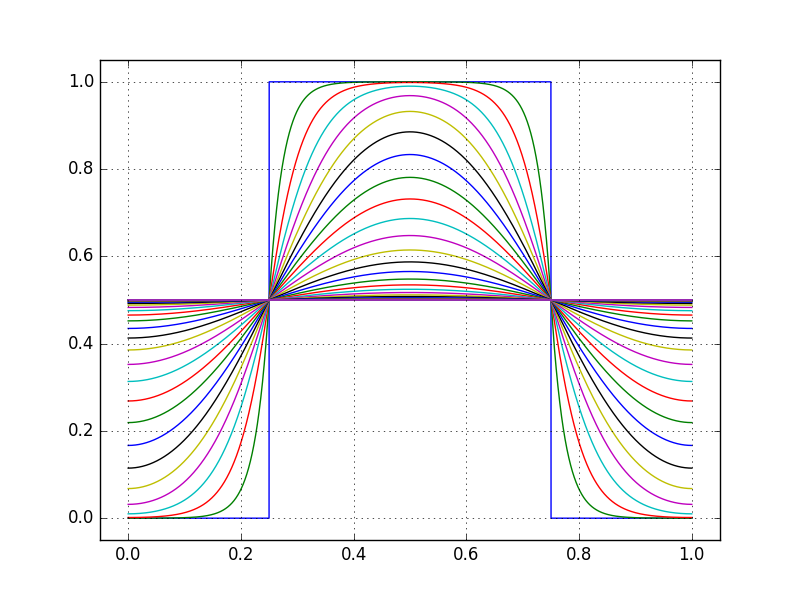
\includegraphics[width=1\textwidth]{solution-plot.png}
\caption{\label{fig:solution-plot}Distribution of heat over time}
\end{figure}


\begin{appendix}
   \newpage
   \addappheadtotoc
   \appendixpage
   \section{Python Code}
   \sloppy
   Python solve Heat Equation PDE (\ref{fig:solution-plot})
   \lstinputlisting[language=Python,style=custom_py_style]{/home/ian/Desktop/ACM41000-Uncertainty-Quantification/assignment2/assignment2.py}
\end{appendix}


\end{document}
